\begin{frame}{Desagregaci\'on del Sector P\'ublico Consolidado}
\centering
\begin{tikzpicture}[node distance=0.5cm and 0.5cm, every node/.style={align=center},
  box/.style={rectangle, draw, rounded corners, text width=3cm, minimum height=0.7cm},
  level/.style={rectangle, draw, text width=3cm, minimum height=0.7cm}]

\node[box, fill=blue!10] (spc) {\tiny{Sector P\'ublico Consolidado}};

\node[level, below left=of spc] (spf) {\tiny{Sector Público Financiero}};
\node[level, fill=green!10, below =of spc] (spnf) {\tiny{Sector Público No Financiero}};


\node[level, fill=green!10, below=of spnf] (gg) {\tiny{Gobierno General}};
\node[level, below left =of spnf] (eepp) {\tiny{Empresas Públicas}};


\node[level, fill=red!10, below left=of gg] (gnc) {\tiny{Gobierno Nacional Central}};
\node[level, fill=red!10, below =of gg] (et) {\tiny{Entidades Territoriales}};
\node[level, fill=red!10, below right =of gg] (ss) {\tiny{Seguridad Social}};

%\node[level, below left=of ss] (salud) {\tiny{Salud}};
%\node[level, below right =of ss] (pensiones) {\tiny{Pensiones}};

\node[box, fill=blue!10] (spc) {Sector P\'ublico Consolidado};

% Conexiones directas desde SPC
\draw[->] (spc) -- (spf);
\draw[->] (spc) -- (spnf);

\draw[->] (spnf) -- (gg);
\draw[->] (spnf) -- (eepp);

\draw[->] (gg) -- (gnc);
\draw[->] (gg) -- (et);
\draw[->] (gg) -- (ss);
\end{tikzpicture}
\end{frame}


\begin{frame}{Definición de balance en billones de pesos}
\begin{equation*}
B = T - G
\end{equation*}
\vspace{0.5em}
\begin{itemize}
  \item $B$: Balance fiscal en billones de pesos
  \item $T$: Ingresos totales del gobierno
  \item $G$: Gasto total del gobierno (incluye intereses)
\end{itemize}
\end{frame}

\begin{frame}{Relación entre déficit y balance}
\begin{equation*}
\text{Déficit} = -B
\end{equation*}
\vspace{0.5em}
\begin{itemize}
  \item $B$: Balance fiscal en billones de pesos
  \item Si $B < 0$, el gobierno tiene un déficit
  \item Si $B > 0$, el gobierno tiene un superávit
  %\item Por convención, el déficit es una magnitud positiva
\end{itemize}
\end{frame}


\begin{frame}{PIB de Colombia en 2026}
\begin{itemize}
  \item \textbf{PIB nominal proyectado de Colombia en 2026:} \\
  \quad \$1,998 billones de pesos corrientes
  
  \vspace{1em}
  \item \textbf{1 punto del PIB:} \\
  \quad \$1,998 billones × 1\% = \textbf{\$19.98 billones de pesos}
  
  \vspace{1em}
  \item Esta equivalencia permite interpretar los saldos fiscales expresados como porcentaje del PIB en términos absolutos.
\end{itemize}
\end{frame}


\begin{frame}{Definición de balance como porcentaje del PIB}
\begin{equation*}
b = t - g
\end{equation*}
\vspace{0.5em}
\begin{itemize}
  \item $b$: Balance fiscal como porcentaje del PIB
  \item $t$: Ingresos totales del gobierno
  \item $g$: Gasto total del gobierno (incluye intereses)
\end{itemize}
\end{frame}

\begin{frame}{Relación entre niveles y proporciones del PIB}
\begin{align*}
b &= \frac{B}{PIB} = \frac{T - G}{PIB} = \frac{T}{PIB} - \frac{G}{PIB} = t - g
\end{align*}
\vspace{0.5em}
\begin{itemize}
  \item $b$: Balance fiscal como \% del PIB
  \item $B$: Balance fiscal en billones de pesos
  \item $t = \frac{T}{PIB}$: Ingresos como \% del PIB
  \item $g = \frac{G}{PIB}$: Gasto como \% del PIB
\end{itemize}
\end{frame}

\begin{frame}{Desagregaci\'on del Sector P\'ublico Consolidado}
\centering
\begin{tikzpicture}[node distance=0.5cm and 0.5cm, every node/.style={align=center},
  box/.style={rectangle, draw, rounded corners, text width=3cm, minimum height=0.7cm},
  level/.style={rectangle, draw, text width=3cm, minimum height=0.7cm}]

\node[box, fill=blue!10] (spc) {\tiny{Sector P\'ublico Consolidado}};

\node[level, below left=of spc] (spf) {\tiny{Sector Público Financiero}};
\node[level, fill=green!10, below =of spc] (spnf) {\tiny{Sector Público No Financiero}};


\node[level, fill=green!10, below=of spnf] (gg) {\tiny{Gobierno General}};
\node[level, below left =of spnf] (eepp) {\tiny{Empresas Públicas}};


\node[level, fill=red!10, below left=of gg] (gnc) {\tiny{Gobierno Nacional Central}};
\node[level, fill=red!10, below =of gg] (et) {\tiny{Entidades Territoriales}};
\node[level, fill=red!10, below right =of gg] (ss) {\tiny{Seguridad Social}};

%\node[level, below left=of ss] (salud) {\tiny{Salud}};
%\node[level, below right =of ss] (pensiones) {\tiny{Pensiones}};

\node[box, fill=blue!10] (spc) {Sector P\'ublico Consolidado};

% Conexiones directas desde SPC
\draw[->] (spc) -- (spf);
\draw[->] (spc) -- (spnf);

\draw[->] (spnf) -- (gg);
\draw[->] (spnf) -- (eepp);

\draw[->] (gg) -- (gnc);
\draw[->] (gg) -- (et);
\draw[->] (gg) -- (ss);
\end{tikzpicture}
\end{frame}

\begin{frame}[t]{Balance fiscal del Sector Público No Financiero, 2025}

\vspace{-0.4em}

\begin{table}
\centering

{\small Balances por subsector (\% del PIB)}

\vspace{0.4em}

\fontsize{5.2}{5.9}\selectfont
\renewcommand{\arraystretch}{1.05}
\setlength{\tabcolsep}{2pt}

\begin{tabular}{
    @{}p{0.35\linewidth}r
    @{\hspace{6pt}}
    p{0.35\linewidth}r@{}
}

\hline
\textbf{Subsector} & \textbf{2025*}
& \textbf{Subsector} & \textbf{2025*} \\
\hline

\textbf{Sector Público No Financiero (SPNF)}
& \textbf{-6.7}
& Seguridad social
& 0.4
\\

\textbf{Gobierno General (GG)}
& \textbf{-6.1}
& \textbf{Empresas}
& \textbf{-0.2}
\\

\hspace{0.5em} Gobierno central
& -6.1
& \hspace{0.5em} Empresas nacionales
& 0.0
\\

\hspace{1em} Gobierno Nacional Central (GNC)
& -6.4
& \hspace{1em} Sector eléctrico
& 0.0
\\

\hspace{1em} Resto del Gobierno Central
& 0.2
& \hspace{1em} Ecopetrol
& 0.0
\\

\hspace{1.5em} Establecimientos públicos
& 0.0
& \hspace{1em} Telecom
& 0.0
\\

\hspace{1.5em} Agencia Nacional de Hidrocarburos (ANH)
& -0.1
& \hspace{0.5em} Empresas locales
& -0.2
\\

\hspace{1.5em} Fondo Nacional del Café (FNC)
& 0.0
& \hspace{1em} Empresas Públicas de Medellín (EPM)
& -0.2
\\

\hspace{1.5em} FEPC
& 0.2
& \hspace{1em} ETB
& 0.0
\\

\hspace{1.5em} Fondes
& 0.0
& \hspace{1em} Metro de Medellín
& 0.0
\\

\hspace{0.5em} Regionales y locales
& -0.4
& \hspace{1em} EAAB
& 0.0
\\

\hspace{1em} Administraciones centrales de las ET
& -0.2
& \hspace{1em} Empresas Municipales de Cali (Emcali)
& 0.0
\\

\hspace{1em} Sistema General de Regalías (SGR)
& -0.2
& \textbf{Sector Público No Modelado (SPNM)}
& \textbf{-0.4}
\\

\hspace{1em} Fondo de Ahorro y Estabilización Petrolera (FAEP)
& 0.0
& \textbf{Balance primario del SPNF}
& \textbf{-3.4}
\\

\hline

\end{tabular}

\end{table}

\vfill


\end{frame}

\begin{frame}{Definiciones: gasto primario y balance primario}
\begin{align*}
GP &= G - I \\
P &= T - GP = T - (G - I) = B + I
\end{align*}
\vspace{0.5em}
\begin{itemize}
  \item $GP$: Gasto primario en billones de pesos (excluye intereses)
  \item $G$: Gasto total del gobierno (incluye intereses)
  \item $I$: Pago de intereses en billones de pesos
  \item $P$: Balance primario en billones de pesos
  \item $T$: Ingresos totales del gobierno
  \item $B$: Balance fiscal total en billones de pesos
\end{itemize}
\end{frame}

\begin{frame}{Gasto primario y balance primario como \% del PIB}
\begin{align*}
gp &= g - i \\
p &= t - gp = t - (g - i) = b + i
\end{align*}
\vspace{0.5em}
\begin{itemize}
  \item $gp$: Gasto primario como porcentaje del PIB
  \item $g$: Gasto total del gobierno como \% del PIB
  \item $i$: Intereses como \% del PIB
  \item $p$: Balance primario como \% del PIB
  \item $t$: Ingresos totales como \% del PIB
  \item $b$: Balance fiscal total como \% del PIB
\end{itemize}
\end{frame}

\begin{frame}{Recordatorio contable: ¿Qué es el patrimonio?}
\begin{equation*}
\textbf{Patrimonio} = \text{Activos} - \text{Pasivos}
\end{equation*}

\vspace{1em}
\begin{itemize}
  \item \textbf{Activos:} Bienes y derechos que posee el Estado (efectivo, inversiones, infraestructura, cuentas por cobrar, etc.)
  \item \textbf{Pasivos:} Obligaciones del Estado (deuda pública, cuentas por pagar, etc.)
  \item \textbf{Patrimonio:} Es la diferencia entre lo que el Estado posee y lo que debe.
\end{itemize}

\vspace{1em}
\textit{El balance fiscal refleja el cambio en ese patrimonio, excluyendo operaciones que solo modifican activos y pasivos sin efecto patrimonial.}
\end{frame}


\begin{frame}{¿Por qué las amortizaciones no son gasto público?}
\textbf{El balance mide el cambio en el patrimonio :}
\begin{equation*}
\text{Balance} = \text{Ingresos} - \text{Gastos}
\end{equation*}

\vspace{1em}
\textbf{Implicación contable:}
\begin{itemize}
  \item Solo se incluyen operaciones que afectan el \textbf{patrimonio}.
  \item Las \textbf{amortizaciones} (pago del principal de la deuda) reducen un activo...
  \item ... pero también reducen un pasivo (deuda) en el mismo monto.
  \item Por lo tanto, no afectan el patrimonio.
  \item Como consecuencia, no se consideran gasto.
\end{itemize}
\end{frame}

\begin{frame}
\textbf{En cambio, los intereses sí son gasto:}
\begin{itemize}
  \item Son un pago por el uso de recursos prestados.
  \item Disminuyen el patrimonio neto sin reducir pasivos.
\end{itemize}
\end{frame}

\begin{frame}{Ejercicio: ¿Qué parte de mi cuota hipotecaria es gasto?}
\textbf{Pago mensual:} \$6 millones

\vspace{0.5em}
\begin{itemize}
  \item \$4 millones corresponden a \textbf{intereses} → \textbf{Gasto}
  \item \$2 millones corresponden a \textbf{amortización del capital} → \textbf{No es gasto}
\end{itemize}

\vspace{1em}
\textbf{Interpretación:}
\begin{itemize}
  \item Los intereses reducen mi efectivo disponible pero no reducen mi deuda → reducen mi patrimonio →se consideran gasto.
  \item La amortización reduce mi efectivo disponible (activo) pero también reduce mi deuda (pasivo) → no afecta patrimonio! → no es gasto 
\end{itemize}

\vspace{1em}
\textit{Lo mismo aplica para las cuentas fiscales del gobierno.}
\end{frame}

\begin{frame}{Ejercicio: ¿Vender mi apartamento es un ingreso?}
\textbf{Supongamos:} Vendo mi apartamento por \$500 millones.

\vspace{1em}
\begin{itemize}
  \item Aumenta mi \textbf{activo líquido} (efectivo) en \$500 millones.
  \item Disminuye mi \textbf{activo fijo} (apartamento) en \$500 millones.
  \item \textbf{No cambia mi patrimonio neto.}
\end{itemize}

\vspace{1em}
\textbf{Conclusión:} No es un ingreso económico.  
Es una \textbf{reorganización de activos}, no un aumento de riqueza.

\vspace{1em}
\textit{En contabilidad pública, vender un activo (como una propiedad del Estado) no \textbf{debería} registrarse como ingreso fiscal.}
\end{frame}

\begin{frame}{Ejercicio: ¿Pedir prestado dinero es un ingreso?}
\textbf{Supongamos:} Pido prestados \$100 millones a un banco.

\vspace{1em}
\begin{itemize}
  \item Mi \textbf{activo} (efectivo disponible) aumenta en \$100 millones.
  \item Mi \textbf{pasivo} (deuda con el banco) también aumenta en \$100 millones.
  \item \textbf{No cambia mi patrimonio neto}.
\end{itemize}

\vspace{1em}
\textbf{Conclusión:}
\begin{itemize}
  \item No es un ingreso real.
  \item Es una \textbf{operación financiera}: financia mis gastos, pero no me vuelve más rico.
\end{itemize}

\vspace{1em}
\textit{Lo mismo aplica en las finanzas públicas: el endeudamiento no es ingreso fiscal.}
\end{frame}

\begin{frame}{Ejercicio: ¿La venta de ISA fue un ingreso fiscal?}
\textbf{En 2021, el Gobierno vendió su participación en ISA por \$14,2 billones.}

\vspace{1em}
\begin{itemize}
  \item Se redujo un \textbf{activo financiero} del Estado (participación accionaria en ISA).
  \item Se incrementó el \textbf{efectivo disponible} (activo líquido).
  \item \textbf{No cambió el patrimonio neto}: solo se intercambió un activo por otro.
\end{itemize}

\vspace{1em}
\textbf{Conclusión:}  
\begin{itemize}
  \item No fue un ingreso fiscal corriente.
  \item Se registró como una \textbf{fuente de financiamiento}, no como ingreso que mejora el balance fiscal.
\end{itemize}

\vspace{1em}
\textit{La venta de activos públicos no debe confundirse con un aumento permanente en los ingresos del gobierno.}
\end{frame}

\begin{frame}{Ingresos del GNC \$ MM}
\begin{center}
\adjustbox{max width=0.99\textwidth}{
  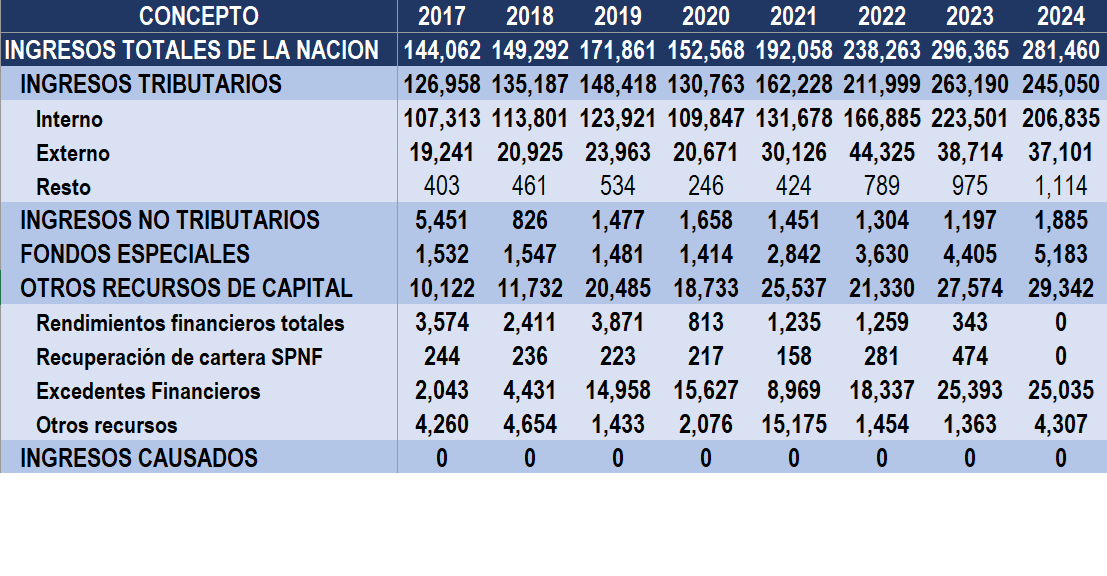
\includegraphics{assets/IngresosGNC.png}
}
\end{center}
\end{frame}



\begin{frame}{Pero el Gobierno hizo trampa...}
\textbf{¿Qué pasó realmente con la venta de ISA?}

\vspace{1em}
\begin{itemize}
  \item Aunque la operación fue una \textbf{enajenación de activos}, el Gobierno la registró como un \textbf{ingreso de capital}.
  \item Esto permitió mostrar un \textbf{mejor balance fiscal} en 2021.
  \item La operación no correspondía a una fuente estructural ni a un ingreso tributario.
  \item Fue una forma de \textbf{mejorar artificialmente} el resultado fiscal, sin mejorar la sostenibilidad de largo plazo.
\end{itemize}

\vspace{1em}
\textit{Contablemente cuestionable, fiscalmente riesgoso.}
\end{frame}

\begin{frame}{Contabilidad presupuestal vs. contabilidad fiscal en Colombia}
\textbf{En Colombia, la contabilidad presupuestal y la contabilidad fiscal no coinciden.}

\vspace{1em}
\textbf{Contabilidad presupuestal:}
\begin{itemize}
  \item Se basa en el \textbf{Presupuesto General de la Nación (PGN)}.
  %\item Registra compromisos y apropiaciones aprobadas.
  \item Clasifica el gasto según \textbf{funcionamiento}, \textbf{inversión} y \textbf{servicio de la deuda}.
  \item Es una contabilidad jurídica y operativa.
\end{itemize}

\vspace{1em}
\textbf{Contabilidad fiscal:}
\begin{itemize}
  \item Sigue criterios del \textbf{Manual de Estadísticas de Finanzas Públicas (MEFP)} del FMI.
  \item Se enfoca en el  \textbf{cambio en el patrimonio}.
  \item (En teoría) excluye operaciones financieras como amortizaciones, prestamos o enajenación de activos.
\end{itemize}

\end{frame}



